\section{Materials and methods}
\label{sec:methods}

\subsection{Scope and workflow}
\label{sec:mm-workflow}

PLECTA turns a binary strand-axis mask into a set of overlap-aware strand
instances, as shown in the workflow diagram in Figure~\ref{fig:scope}. For
validation and comparison against a known ground truth, the mask can be
generated synthetically; masks derived from SEM images are also tested in this
paper (Sections~\ref{sec:mm-synth} and~\ref{sec:mm-real}). PLECTA then builds a graph
of arms, stubs and junction nodes and fits a tangent and curvature frame to
each stub (Section~\ref{sec:mm-graph}). It scores candidate continuations
(Section~\ref{sec:mm-cost}), solves exact partial matchings at junctions and
across admissible gaps over eight frame-refitting rounds
(Section~\ref{sec:mm-matching}), and converts the accepted links into
overlapping strand instances (Section~\ref{sec:mm-output}). Given a paired
greyscale image, downstream stages estimate strand width and render ribbons
(Section~\ref{sec:mm-stage4}) and infer depth order at crossings
(Section~\ref{sec:mm-depth}).

\begin{figure}[!ht]
    \centering
    % ---------------------------------------------------------------------------
%  Figure 1.  Drawn in TikZ, in the document's own face at the document's own
%  size, replacing the matplotlib figures/fig_pipeline_scope.pdf whose
%  generator now writes to figures/archive/.
%
%  Layout notes:
%    * Row 2 runs right to left, so the reading order over both rows is the
%      order the method runs in: graph, frames, junction matching, gap
%      bridging, output.
%    * The dashed boundary fits only the four method stages.  The input mask
%      and the output box share column 1, so fitting either would sweep the
%      rectangle over the other; with both outside, the two arrows crossing
%      the dashed edge are the method's input and output.
%    * The depth row is grey and ends at the global order; layer and height
%      bookkeeping is left to the text (Section 2.5.2).
%    * All three depth boxes sit on the top grid's own columns, so the arrow
%      from the output box down to the first of them is exactly vertical.
%
%  Requires the pk vocabulary defined in main.tex's preamble.
% ---------------------------------------------------------------------------
\begin{tikzpicture}[pk, x=1mm, y=1mm]

  % ---- the core, two rows of three ---------------------------------------
  \node[io=38mm]    (mask)   at ( 27,   0) {Binary axis mask};
  \node[stage=38mm] (graph)  at ( 81.5, 0) {Arms, stubs and\\junction nodes};
  \node[stage=38mm] (frame)  at (136,   0) {Tangent and curvature\\frame at each stub};

  \node[io=38mm]    (out)    at ( 27,  -26) {Overlapping\\instance layers};
  \node[stage=38mm] (bridge) at ( 81.5,-26) {Gated bridging\\of mask gaps};
  \node[stage=38mm] (match)  at (136,  -26) {Exact partial matching\\at each junction};

  \draw[flow] (mask)   -- (graph);
  \draw[flow] (graph)  -- (frame);
  \draw[flow] (frame)  -- (match);
  \draw[flow] (match)  -- (bridge);
  \draw[flow] (bridge) -- (out);

  % ---- the round schedule, drawn as the cycle it is ----------------------
  \draw[loop] (bridge.north) -- (graph.south);

  % ---- the evaluated boundary -------------------------------------------
  \begin{scope}[on background layer]
    \node[scope, fit=(graph)(frame)(match)(bridge)] (core) {};
  \end{scope}

  % ---- the depth stage ----------------------------------------------------
  %  Centred to the right of the output arrow's x so the two never cross.
  \node[ext=38mm] (cross) at ( 27,  -52) {Crossings in\\projection};
  \node[ext=38mm] (ou)    at ( 81.5,-52) {Over or under,\\from brightness};
  \node[ext=38mm] (order) at (136,  -52) {One global order,\\cycles removed};

  \draw[flowsoft] (cross) -- (ou);
  \draw[flowsoft] (ou)    -- (order);
  \draw[flowsoft] (out.south) -- (cross.north);

\end{tikzpicture}

    \caption{Scope of PLECTA. The dashed grouping stage maps a binary axis mask
    to overlapping instances; the loop denotes eight rounds of frame refitting
    and matching. The grey branch uses a paired greyscale image to infer depth
    order without changing strand identity.}
    \label{fig:scope}
\end{figure}

\subsection{Synthetic data}
\label{sec:mm-synth}

Strand centrelines are generated as random walks with Gaussian-smoothed
angular increments, producing gradual bends with controllable curvature.
Strands are placed at random positions and orientations until their combined
full-width area reaches the target coverage of 20, 30, 40, 50 or 60\,\% of
the image area.
Each synthetic scene provides strand centrelines $\mathcal C_k$, their
corresponding pixel sets $\Omega_k$, and four image representations: a
one-pixel axis mask; a version with gaps and raster irregularities; a
full-width foreground mask; and an SEM-like greyscale image with
strand-specific brightness, gradual intensity variation, blur and background
noise. For depth evaluation (Section~\ref{sec:mm-depth}), a depth-resolved
variant assigns strand heights and radii, prevents interpenetration and
renders the scene from above. Occlusion, depth-dependent defocus and width
broadening are included, with imaging cues randomised independently so that
no single cue reliably determines crossing order.


\subsection{CNT SEM data and mask sources}
\label{sec:mm-real}

\PlectaRealFieldCountWord{} CNT-sheet SEM fields were analysed, each comprising
$1536\times1024$ pixels: B58\_100, B58\_110 and B58\_300, containing
\PlectaBFiveEightOneZeroZeroReferenceCount{},
\PlectaBFiveEightOneOneZeroReferenceCount{} and
\PlectaBFiveEightThreeZeroZeroReferenceCount{} annotated bundles, respectively.
Each strand annotation represents a visible bundle, as individual nanotubes
are unresolved at this magnification. The horizontal field width was
$1.66~\um$, corresponding to $1.08~\mathrm{nm\,px^{-1}}$. Images were acquired
using a Thermo Fisher Helios 5~UX DualBeam with an Elstar field-emission column
in immersion mode and a through-lens detector, at 2.00\,kV, 400\,pA and a
working distance of 4.3\,mm. Each frame integrated 35 passes at a dwell time
of 100\,ns with drift correction.

The first author (O.A.) and an independent second annotator each annotated
all \PlectaInterAnnotatorFieldCount{} fields using an in-house tool that permits
overlapping strand masks. Ridge snapping and spline smoothing assisted
tracing, while strand connections and suggested gap bridges required manual
decisions. Scores are reported separately against each annotator, with their
agreement discussed in
Section~\ref{sec:limitations}. Supplementary Section~S7 describes the
annotation procedure.

Two input masks were evaluated for each field: a skeletonised mask derived
from the first author's reference and an automatically generated mask from the
upstream CycleGAN/nnU-Net segmentation (Section~\ref{sec:res-qualitative})
\citep{ruehle2021workflow,isensee2021nnunet}. These inputs assess reconstruction
from manually curated and automatically extracted strand axes, respectively.
The automatic segmentation required no manual annotations for training or
inference.

Strand reconstruction was evaluated on the common centreline fragments
visible within each input mask,
using the metrics defined in Section~\ref{sec:mm-metrics}.


\subsection{PLECTA reconstruction}
\label{sec:mm-plecta}

Starting from a binary strand mask, PLECTA reconstructs individual strands by
resolving connections through junctions and across gaps. The following
subsections describe the main steps: constructing the skeleton graph, scoring
candidate connections and selecting compatible links, with iterative
refinement as longer strands are assembled. For an input mask
$M\in\{0,1\}^{H\times W}$, the output is a set of strand instances
$\{I_1,\ldots,I_N\}$, with $I_n\subseteq F=\{x:M(x)=1\}$; crossing pixels
may belong to multiple instances. Reconstruction uses the mask alone, while
subsequent width and depth estimates also use the greyscale image
(Section~\ref{sec:mm-image}).

\subsubsection{Skeleton graph and local geometry}
\label{sec:mm-graph}

PLECTA skeletonises the input mask using the Zhang--Suen thinning algorithm
\citep{zhang1984thinning} and removes short spurs. Pixels where three or more
skeleton branches meet are grouped into junction clusters, with nearby
clusters merged into a single \emph{node}. This accounts for crossings that
span several pixels or lie too close together to resolve separately. The
remaining strand segments form \emph{arms}, each with a \emph{stub} at either
end.

Each stub is characterised by its tip position, outward tangent
($\mathbf{t}$) and signed curvature ($\kappa$), estimated from a short segment
of the adjoining strand (Figure~\ref{fig:cost}a). Subscripts identify the stub,
so $\mathbf{t}_a$ and $\kappa_a$ denote the tangent and curvature of stub $a$.
Stubs with insufficient support for a reliable direction estimate are marked
as unreliable. As arms are linked into longer chains, these estimates are
updated using the additional strand geometry.

\subsubsection{Pairing cost function}
\label{sec:mm-cost}

The cost $C_{ab}$ of linking stubs $a$ and $b$ combines directional alignment,
chord alignment and curvature continuity (Equation~\ref{eq:cost};
Figure~\ref{fig:cost}). The reversal angle $\theta$, measured between
$\mathbf{t}_a$ and $-\mathbf{t}_b$, is zero when the outward tangents form a
straight continuation. The chord angles $\varphi_a$ and $\varphi_b$ measure
how far each tangent turns towards the opposite tip, penalising lateral
offset between otherwise aligned arms. The curvature mismatch
$\lvert\kappa_a+\kappa_b\rvert$ penalises changes in bending; the sum reflects
the opposite orientations of the outward frames. Gap links also incur a
penalty for tip separation $d$:
\begin{equation}
  C_{ab}=w_d\,\theta
        +w_t\,q(d)\,(\varphi_a+\varphi_b)
        +w_\ell\,\frac{d}{\ell_0}
        +30\,w_\kappa\,\lvert\kappa_a+\kappa_b\rvert,
  \qquad q(d)=\min\!\left(1,\tfrac{d}{d_0}\right),
  \label{eq:cost}
\end{equation}
where $w_d$, $w_t$, $w_\ell$ and $w_\kappa$ weight the four terms, and
$\ell_0$ normalises the gap distance. Junction links set $w_\ell=0$.

The reversal angle $\theta$ is independent of the tip-to-tip chord and remains
useful when nearby tips make the chord direction sensitive to pixel
quantisation. The factor $q(d)$ therefore reduces the chord-angle contribution
at separations below $d_0$. The weights, distance scales $\ell_0$ and $d_0$,
and curvature scaling factor of 30 are fixed parameters listed in
\supprecon{}. These costs quantify the suitability of individual connections;
the next step selects a compatible set of links.

\begin{figure}[tbp]
    \centering
    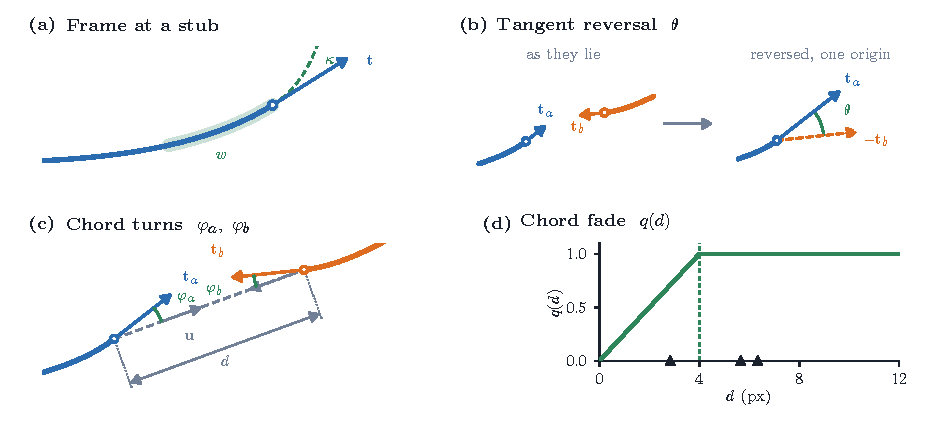
\includegraphics[width=\linewidth]{figures/fig_plecta_frame_cost.pdf}
    \caption{The stub frame and the terms of the pairing cost.
    \textbf{(a)}~The least-squares arclength fit over window $w$, read outward
    from the tip at $s=0$, giving outward tangent $\mathbf{t}$ and signed
    curvature $\kappa$; quadratic when the span allows, linear otherwise.
    \textbf{(b)}~$\theta$, in the two steps its definition takes: the outward
    tangents where they lie, then the same pair with $\mathbf{t}_b$ reversed and
    both read from one origin. A perfect continuation makes them antiparallel,
    so $\theta=0$. \textbf{(c)}~The chord turns $\varphi_a$, $\varphi_b$ onto the
    chord $\mathbf{u}$ joining the tips. \textbf{(d)}~The fade $q(d)$ against tip
    separation; triangles mark the six real separations at the crossing of
    Figure~\ref{fig:matching}.}
    \label{fig:cost}
\end{figure}

\subsubsection{Candidate selection and iterative matching}
\label{sec:mm-matching}

Using the costs from Equation~\ref{eq:cost}, PLECTA selects links jointly so
that no stub is assigned to more than one connection. Leaving stub $i$
unmatched incurs a penalty $p_i$. Connecting stubs $i$ and $j$ avoids both
unmatched penalties but incurs the linking cost $C_{ij}$ defined in
Equation~\ref{eq:cost}. The net benefit of the connection is therefore
$p_i+p_j-C_{ij}$. A link is admissible only if $C_{ij}<p_i+p_j$.
Exact maximum-weight partial matching then selects the set of disjoint stub
pairs $\Gamma$ with the greatest total benefit:
\begin{equation}
  \max_{\Gamma}\sum_{(i,j)\in\Gamma}
  \bigl(p_i+p_j-C_{ij}\bigr).
  \label{eq:matching}
\end{equation}
Each stub can belong to at most one pair or remain unmatched, allowing genuine
strand termination at junctions of any degree. The penalties therefore
determine both candidate admissibility and the preference for linking. Because
competing links are considered together, a locally favourable pair may be
rejected when another combination gives a better overall assignment.

Junction and gap links use different penalties. Gap candidates must also
satisfy distance and angular limits, since they connect strands across missing
image evidence. Figure~\ref{fig:matching} illustrates candidate selection and
matching at junctions and across gaps.

Matching proceeds iteratively, with tangent and curvature estimates updated
along the assembled chains before each round. Early rounds use lower unmatched
penalties and tighter gap-angle limits to restrict uncertain connections.
These constraints gradually relax to their configured values, and the final
round determines the output. \supprecon{} lists the penalties, geometric
limits and iteration schedule; Section~\ref{sec:res-ablation} evaluates joint
matching and the contributions of individual components.

\begin{figure}[tbp]
    \centering
    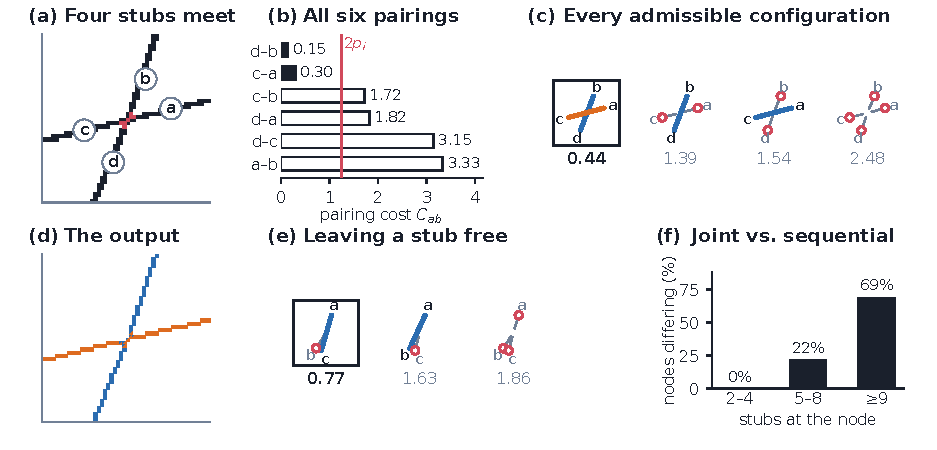
\includegraphics[width=\linewidth]{figures/fig_plecta_exact_matching.pdf}
    \caption{Candidate-link evaluation and matching outcomes, on the nodes
    where the decisions were made. Every arm is the skeleton the numbers were
    measured from, so every angle shown is the one the cost was computed on.
    \textbf{(a)}~Every pairing the admissibility gate allows at a four-arm
    crossing, each scored as a whole: its edge costs plus the penalty
    $p_i=0.62$ of each arm it leaves unmatched. The green frame marks the one
    returned; two further pairs exceed $p_i+p_j=1.24$ and are excluded as
    candidates. \textbf{(b)}~A three-arm node where an admissible edge is
    declined on the total rather than on its own cost. \textbf{(c)}~A gap link,
    which must clear all four gates at once.}
    \label{fig:matching}
\end{figure}

\subsubsection{Strand instance assembly}
\label{sec:mm-output}

After the final matching round, connected components of the accepted arm
links define individual strands. Each strand contains the pixels of its
constituent arms and associated junction clusters, allowing intersecting
strands to share crossing pixels. Accepted gap links connect fragments
belonging to the same strand without adding pixels across the gap. These
strand instances provide the input to the image-based stages described next.

\subsection{Image-informed reconstruction}
\label{sec:mm-image}

The reconstructed strands are combined with the corresponding greyscale image
to estimate their apparent widths and render ribbons
(Section~\ref{sec:mm-stage4}), and to infer crossing order
(Section~\ref{sec:mm-depth}).
These stages preserve the strand identities established during reconstruction
and do not affect the identity scores. They use fixed parameters
(\supprecon{}) and are demonstrated here on SEM images, although the procedure
accepts other greyscale images.

\subsubsection{Width and ribbon rendering}
\label{sec:mm-stage4}

Intensity profiles sampled perpendicular to each strand, away from junctions,
provide estimates of apparent width and brightness, together with uncertainty
and quality indicators. The centreline is then resampled and smoothed, with
accepted gaps interpolated, to render a ribbon at the estimated width.
Junction clusters are excluded from this rendering, and strands remain
separate. The resulting ribbons describe their projected shapes; their
relative positions in depth are estimated in Section~\ref{sec:mm-depth}.

\subsubsection{Depth ordering and height assignment}
\label{sec:mm-depth}

Depth estimation proceeds in three steps: estimating local crossing orders,
combining them into a consistent strand order, and assigning layers and heights.

\textbf{1. Estimate crossing order.} The method assumes that the upper strand
retains its brightness through a crossing, while the lower strand is occluded.
Intensity is sampled through the crossing (the \emph{core}) and along each
strand on either side (the \emph{flanks}), excluding flank pixels occupied by
the other strand (Figure~\ref{fig:depth-evidence}a,b). The pooled core median
$m_c$ is compared with the flank medians $m_i$ and $m_j$; the closer match
indicates the upper strand.

The signed score $s$ summarises this comparison
(Figure~\ref{fig:depth-evidence}c). It compares the two intensity mismatches,
normalised by the larger of $\lvert m_i-m_j\rvert$ and twice the local noise
estimate $\hat\sigma$. Its sign identifies the upper strand and its magnitude
weights the evidence. Crossings with insufficient flank samples or a score
below the threshold in magnitude remain undecided. \suppdepthstage{} gives
the sampling procedure and score equation.

\begin{figure}[!ht]
    \centering
    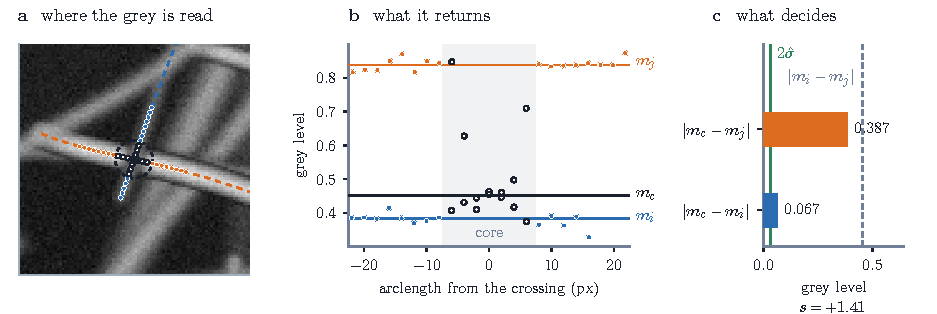
\includegraphics[width=\linewidth]{figures/fig_depth_evidence.pdf}
    \caption{Local depth evidence at a crossing angle of $83.8^{\circ}$,
    selected for clarity. Positions and intensities are taken from the stage
    output. \textbf{(a)}~Core samples (open dots) and flank samples (filled
    dots), with flanks kept clear of the other strand.
    \textbf{(b)}~Intensity along each strand: the pooled core median $m_c$
    is closer to strand $i$'s flank median than to strand $j$'s, supporting
    $i$ as the upper strand. \textbf{(c)}~Intensity mismatches used to
    calculate $s$, normalised by the larger of the flank-median separation
    and twice the local noise estimate (\suppdepthstage{}).}
    \label{fig:depth-evidence}
\end{figure}

\textbf{2. Combine crossing orders.} Local estimates can conflict: $A$ may
lie above $B$, $B$ above $C$, and $C$ above $A$. These relations form a directed
graph whose nodes are strands and whose edges carry weights $\lvert s\rvert$
(Figure~\ref{fig:depth-order}). Within each connected component, a consistent
strand order is sought with the objective of maximising the total weight of
satisfied relations. Crossing orders are updated accordingly.
\suppdepthstage{} describes the ordering procedure.

\begin{figure}[!ht]
    \centering
    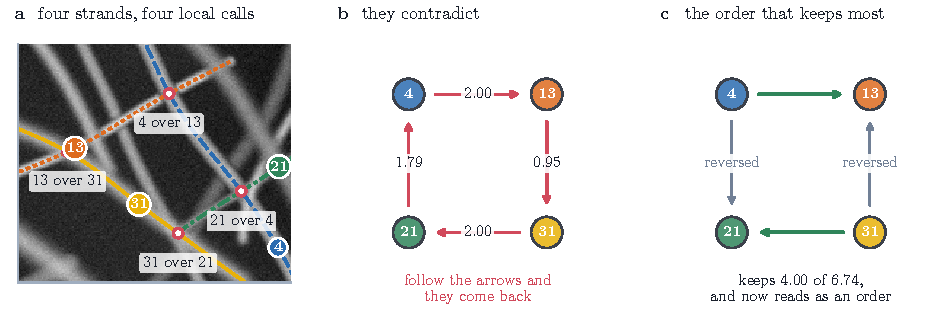
\includegraphics[width=\linewidth]{figures/fig_depth_order.pdf}
    \caption{Resolving contradictory local depth estimates.
    \textbf{(a)}~Four strands and their estimated crossing orders.
    \textbf{(b)}~The corresponding graph, with arrows from the estimated
    upper strand to the lower strand. The directed cycle prevents a
    consistent height assignment. \textbf{(c)}~The selected order retains
    the two highest-weight estimates and reverses the two lowest-weight
    estimates. Reversals are recorded with their original scores. The four
    strands shown belong to a seven-strand scene; layer assignments depend
    on the complete connected component.}
    \label{fig:depth-order}
\end{figure}

\textbf{3. Assign layers and heights.} The corrected relations form a graph
without directed cycles. Its longest path determines the minimum number of
layers needed to respect the crossing orders; strands without ordering
constraints between them may share a layer. Under the compact-stack
assumption, each strand is assigned the lowest height compatible with the
chosen order and the estimated radii, preventing interpenetration.

Without a greyscale image, placement follows the predefined tie-break rather
than measured crossing evidence. Section~\ref{sec:res-depth} evaluates depth ordering
using the measures defined in \suppdepth{}.

\subsection{Metrics and statistical analysis}
\label{sec:mm-metrics}

The primary reconstruction metric is common-fragment pairwise \Fone{}, which
measures whether strand fragments are grouped consistently with the reference.
Each input mask is divided into fragments between crossings, independently of
the reference and predictions. The same assignment rule then gives each
fragment a reference identity and a predicted identity. Pairwise precision
penalises joining fragments from different reference strands, while recall
penalises separating fragments from the same strand.
Figure~\ref{fig:f1-example} illustrates these cases and the conditions under
which the score is undefined.

\begin{figure}[!ht]
    \centering
    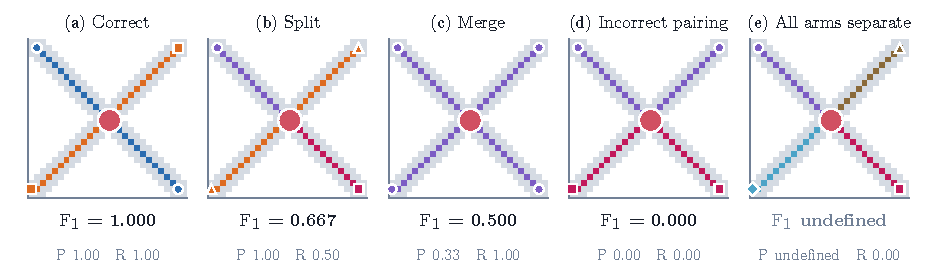
\includegraphics[width=\linewidth]{figures/fig_f1_example.pdf}
    \caption{Pairwise scoring at a crossing. Removing junction pixels (red)
    leaves four arms and six fragment pairs. Tip markers identify arms assigned
    to the same strand. \textbf{(a)}~Reference grouping.
    \textbf{(b)}~A split reduces recall. \textbf{(c)}~A merge reduces precision.
    \textbf{(d)}~Incorrect pairing changes strand identities.
    \textbf{(e)}~Separating every arm produces no predicted positive pair, so
    precision and \Fone{} are undefined.}
    \label{fig:f1-example}
\end{figure}

Because junction pixels are excluded, this metric evaluates strand continuity
through crossings rather than ownership of the crossing pixels themselves.
Strands containing more fragments contribute more pairs and therefore carry
greater weight. We also report the adjusted Rand index and variation of
information \citep{hubert1985comparing,meila2007comparing}, together with
detection \Fone{} and Crossing Fidelity, to characterise complementary aspects
of reconstruction. For the real SEM fields, Join \Fone{} evaluates joining
decisions between nearby fragments, reducing the influence of differences in
fragmentation between mask sources.

Held-out synthetic reconstruction means are accompanied by 95\,\% bootstrap
confidence intervals, with scenes resampled within each density level.
Comparisons between clean and degraded masks preserve scene pairing. For
real SEM data, each image field is treated as one independent sample.
\suppmeasures{} provides the metric definitions, assignment rules and
statistical procedures.
